\section{Database and tools created}
\protect\label{section:tools}

I have developed the following tools and associated software to assist in analysis of the REM observations.

\subsection{Database}
\protect\label{section:database}

I have developed a database (using MySQL) to record the following information.

\begin{enumerate}
\item Observation information, with information about target, filter observation data, airmasss and other information and a link to the corresponding FITS file.
\item Flat file information by month and by filter with link to corresponding FITS file.
\item FITS files (held in compressed format).
\item Object database containing coordinates and details of proper motion, with procedure for finding objects withing
  given arc radius of given point. This also contains an optimal aperture size for each object where appropriate and
  optional data on intensities with various filters.
\item Records of objects found in each FITS image.
\item Records of FITS images rejected, with reason.
\item Calculated ADU counts for each identified object in each image.
\end{enumerate}

In addition I have created a library of access routines for use in Perl and Python programs. A key feature is to be able
to retrieve the visible light filters (\textbf{g}, \textbf{i}, \textbf{r} and \textbf{z} and automatically apply the
appropriate bias and flat files with ``caching'', so that files are only loaded once per run.

\subsection{Software tools}
\protect\label{section:swtools}

At 11:30 each morning, well clear of the nightly observations, I have set up software to get details of new observations,
together with the corresponding FITS files, to get any new flat or bias file details, to find targets and reference
objects in the FITS files, noting any failures with appropriate comments, and to calculate ADU counts for any new
observations.

In addition, I wrote user level tools to list observations for a given day, in total, in summary or with various
restrictions, to display given observation FITS files, automatically inserting markers for found object in each file. to
display light curves with various from all or a selection of the data and to generate periodograms.

In the Fig. \ref{fig:bsheg}, an example is shown of an observation for which no processing has been done (GJ699 is a
shorter name for \bstar, which is used internally). The next figure, Fig. \ref{fig:bsgeg4obj}, shows an example of where 4 reference objects were found.

\begin{figure}[!htbp]
\begin{center}
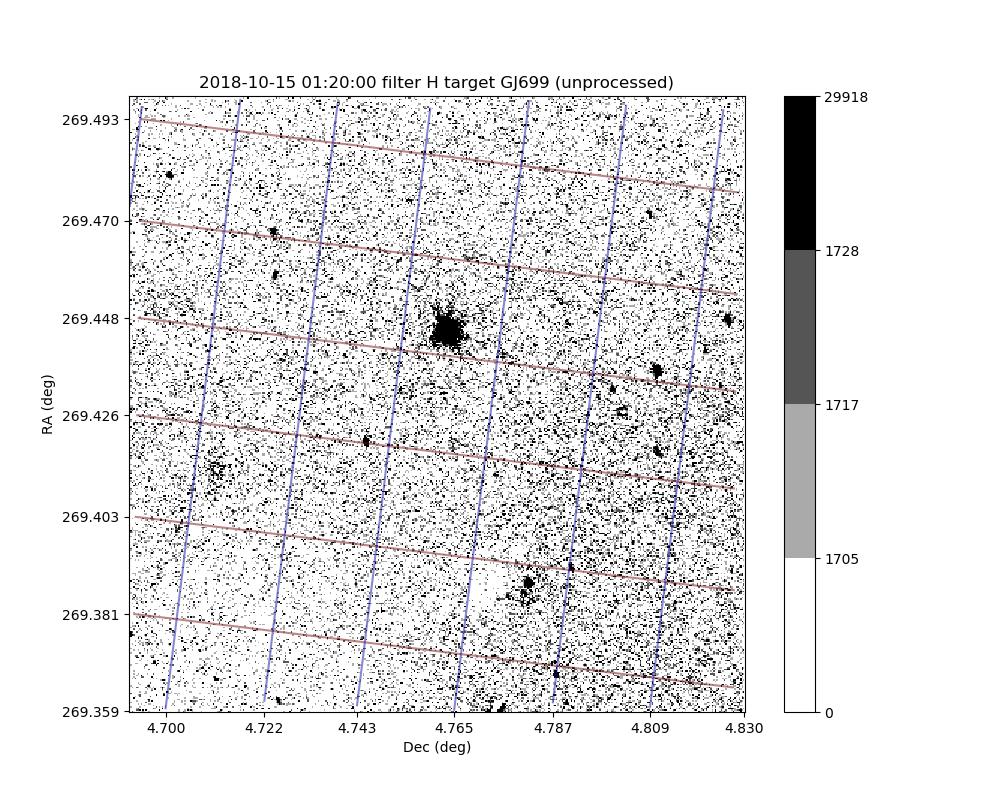
\includegraphics[scale=0.5]{images/bsheg.png} \\
\end{center}   
\caption{The is an example of a figure which has not been searched for target or reference stars. The image is from the Infrared REMIR set for \bstar, on the date shown.}
  \protect\label{fig:bsheg}
\end{figure}

\begin{figure}[!htbp]
\begin{center}
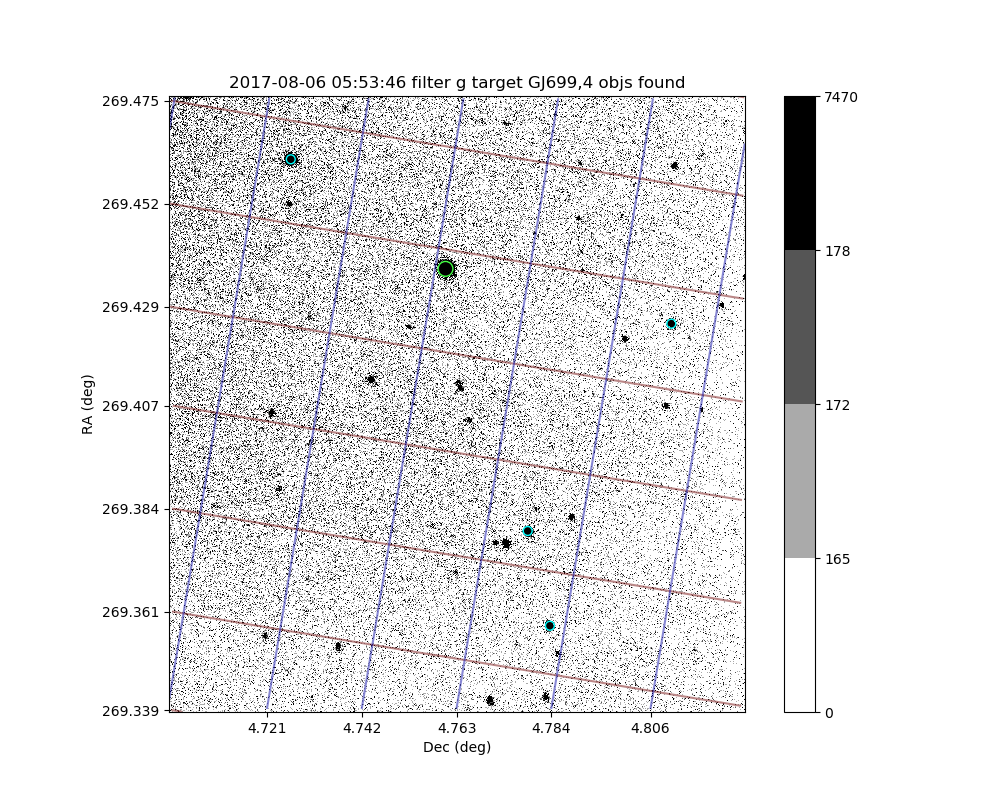
\includegraphics[scale=0.5]{images/bsgeg4obj.png} \\
\end{center}   
\caption{The is an example of a figure which has been searched for target or reference stars, in this case 4 such
  reference stars were found. The circles the objects found, light yellow for the target and light blue for the reference
  objects. Note that the circles shown have different sizes depending on the apertures used, which can be optimised for
  the target.}
\protect\label{fig:bsgeg4obj}
\end{figure}

\subsection{Tunable parameters}
\protect\label{section:tunable}

I put the following key tunable parameters into the database and toolkit.

\begin{description}
\item[Aperture size] Each object in the database can be given an aperture size, represented as a radius in pixels. This
  is desirable as many objects typically have a larger radius in pixels then others.
\item[Default aperture size] This is the radius in pixels to use in calculations where an aperture size is not specified
  for an object. This is currently set to 6 pixels.
  \item[Sky level percentile] The background sky level needs to be subtracted from the ADUs for each of the identified
    objects when calculating the total count. This quantity gives the percentile of the sky level which will be
    subtracted. Default is 50\%, i.e. the median.
    \item[Maximum offset] The maximum offset is the maximum displacement in arc minutes between the reported coordinates
      in the FITS files and the actual coordinates. This needs to be minimal to avoid mis-identification in some cases
      but for some images, notably from REMIR, the reported coordinates are more at variance.
\end{description}
